\documentclass[a4paper,10pt]{article}
\usepackage[utf8x]{inputenc}
\usepackage[T1]{fontenc}
\usepackage[bulgarian]{babel}
\usepackage{graphicx}
\usepackage{alltt}

%opening
\title{Многомерни и битови индекси. Дървовидни структури за многомерни данни в MySQL}
\author{Валентина Динкова, ф.н.71112}

\begin{document}
\maketitle

\newpage
\section{GIS и разширението на MySQL за пространствени данни}
\textbf{GIS} означава Географска Информационна Система и е един от най-очевидните примери за пространствени данни.
\\
\textbf{OGC} (Open Geospatial Consorcium) е организация, която работи по стандартизирането на различни области на GIS.
Един такъв стандарт е и спецификацията за SQL, която определя разширението на SQL базирани релационни бази данни,
 което да използва GIS обекти и операции.
\\
\\
 OGC работи в 4 важни области:
\begin{itemize}
 \item типове данни;
 \item операции;
 \item възможност да се подават като вход и да се извеждат GIS данни;
 \item индексиране на пространствени данни.
\end{itemize}
Друга важна област са метаданните.
\\
\section{Стандартът, използван от почти всички SQL бази данни с пространствено разширение, включително и MySQL}
\begin{center}
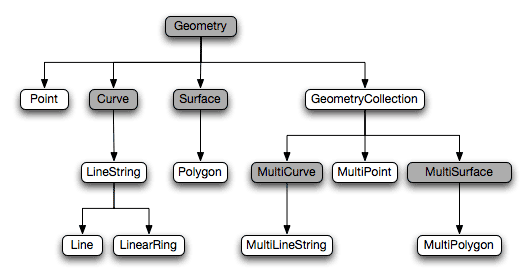
\includegraphics[width=90mm]{gis-datatypes.png}\end{center}
Типовете, отбелязани в сиво са абстракти и обекти от тези типове не могат да се създават.

\section{Пространствени индекси}
Пространствените данни могат да се индексират също както останалите данни в MySQL. Но за да бъде 
индексирането ефективно, се използва пространствен тип индексиране, реализирано чрез R-дървета. 
MySQL използва R-дървета с квадратично разделяне. \\
Не всички engine-и поддържат многомерни индекси.
\subsection{R-дървета с квадратично разделяне}
Добавяме нов запис.
Нека сме намерили листото, където трябва да добавим новия запис и 
нека $M = $ \textit{``брй региони в листо''}.
\begin{enumerate}
\item Избираме 2 от $M+1$ записа да бъдат първите елементи на двете нови листа, като избираме двойката,която би заела
най-много място ако и двата елемента се постават на едно място (двойката при която покриващия регион ще е най-голям).
Намираме тази двойка като от областта покриваща двата записа изваждаме самите записи и искаме тази разлика да е най-голяма.
\begin{center}
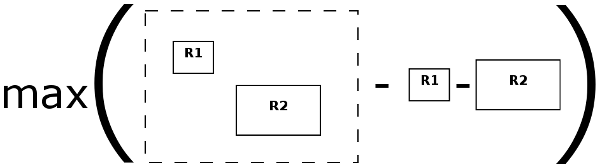
\includegraphics[width=70mm]{Diagram1.png}\end{center}
\item Останалите записи разделяме в двете листа един по един.
На всяка стъпка разширяването, необходимо за добавянето на всеки от оставащите записи към всяко листо се изчислява
и добавеният запис е този, който е показал най-голяма разлика спрямо двете листа.
\end{enumerate}

\subsection{Примери с $MySQL$}
\textbf{Създаваме таблицата $map\_test$, където $loc$ е пространствен атрибут}
\begin{alltt}
mysql> create table map_test
    -> (
    ->   name varchar(100) not null primary key,
    ->   loc  geometry not null,
    -> );
Query OK, 0 rows affected (0.00 sec)
\end{alltt}

\textbf{Добавяме данни}
\begin{alltt}
mysql> insert into map_test values ('One Two', point(1,2));
Query OK, 1 row affected (0.00 sec)

mysql> insert into map_test values ('Two Two', point(2,2));
Query OK, 1 row affected (0.00 sec)

mysql> insert into map_test values ('Two One', point(2,1));
Query OK, 1 row affected (0.00 sec)
\end{alltt}
\newpage

\textbf{Ето как изглежда $map\_test$ сега:}

\begin{alltt}
mysql> select name, AsText(loc) from map_test;
+---------+-------------+
| name    | AsText(loc) |
+---------+-------------+
| One Two | POINT(1 2)  |
| Two Two | POINT(2 2)  |
| Two One | POINT(2 1)  |
+---------+-------------+
3 rows in set (0.00 sec)
\end{alltt}

\textbf{Заявка за проверка коя точка се съдържа в полигона}

\begin{alltt}
mysql> SELECT name, AsText(loc) FROM map_test WHERE
    -> Contains(
    -> GeomFromText('POLYGON((0 0, 0 1, 1 1, 2 0, 0 0))'),
    -> loc) = 1;
+---------+-------------+
| name    | AsText(loc) |
+---------+-------------+
| Two One | POINT(2 1)  |
+---------+-------------+
1 row in set (0.04 sec)
\end{alltt}

\textbf{Сега създаваме пространствен индекс по атрибута $loc$}

\begin{alltt}
mysql> create spatial index ps_index on map_test(loc);
Query OK, 3 rows affected (0.01 sec)
Records: 3  Duplicates: 0  Warnings: 0
\end{alltt}

\textbf{И отново правим същата заявка}

\begin{alltt}
mysql>  SELECT name, AsText(loc) FROM map_test WHERE
    ->  Contains(
    ->  GeomFromText('POLYGON((0 0, 0 1, 1 1, 2 0, 0 0))'),
    ->  loc) = 1;
+---------+-------------+
| name    | AsText(loc) |
+---------+-------------+
| Two One | POINT(2 1)  |
+---------+-------------+
1 row in set (0.00 sec)
\end{alltt}

\end{document}
